\usetikzlibrary{arrows.meta,decorations.pathreplacing}
\begin{frame}[fragile]{}
\begin{tikzpicture}
\tikzset{
    overlay box/.style={fill=white,fill opacity=0.9}
}
\node[overlay,anchor=north west,inner sep=0mm] (base) at (0, 0) {
    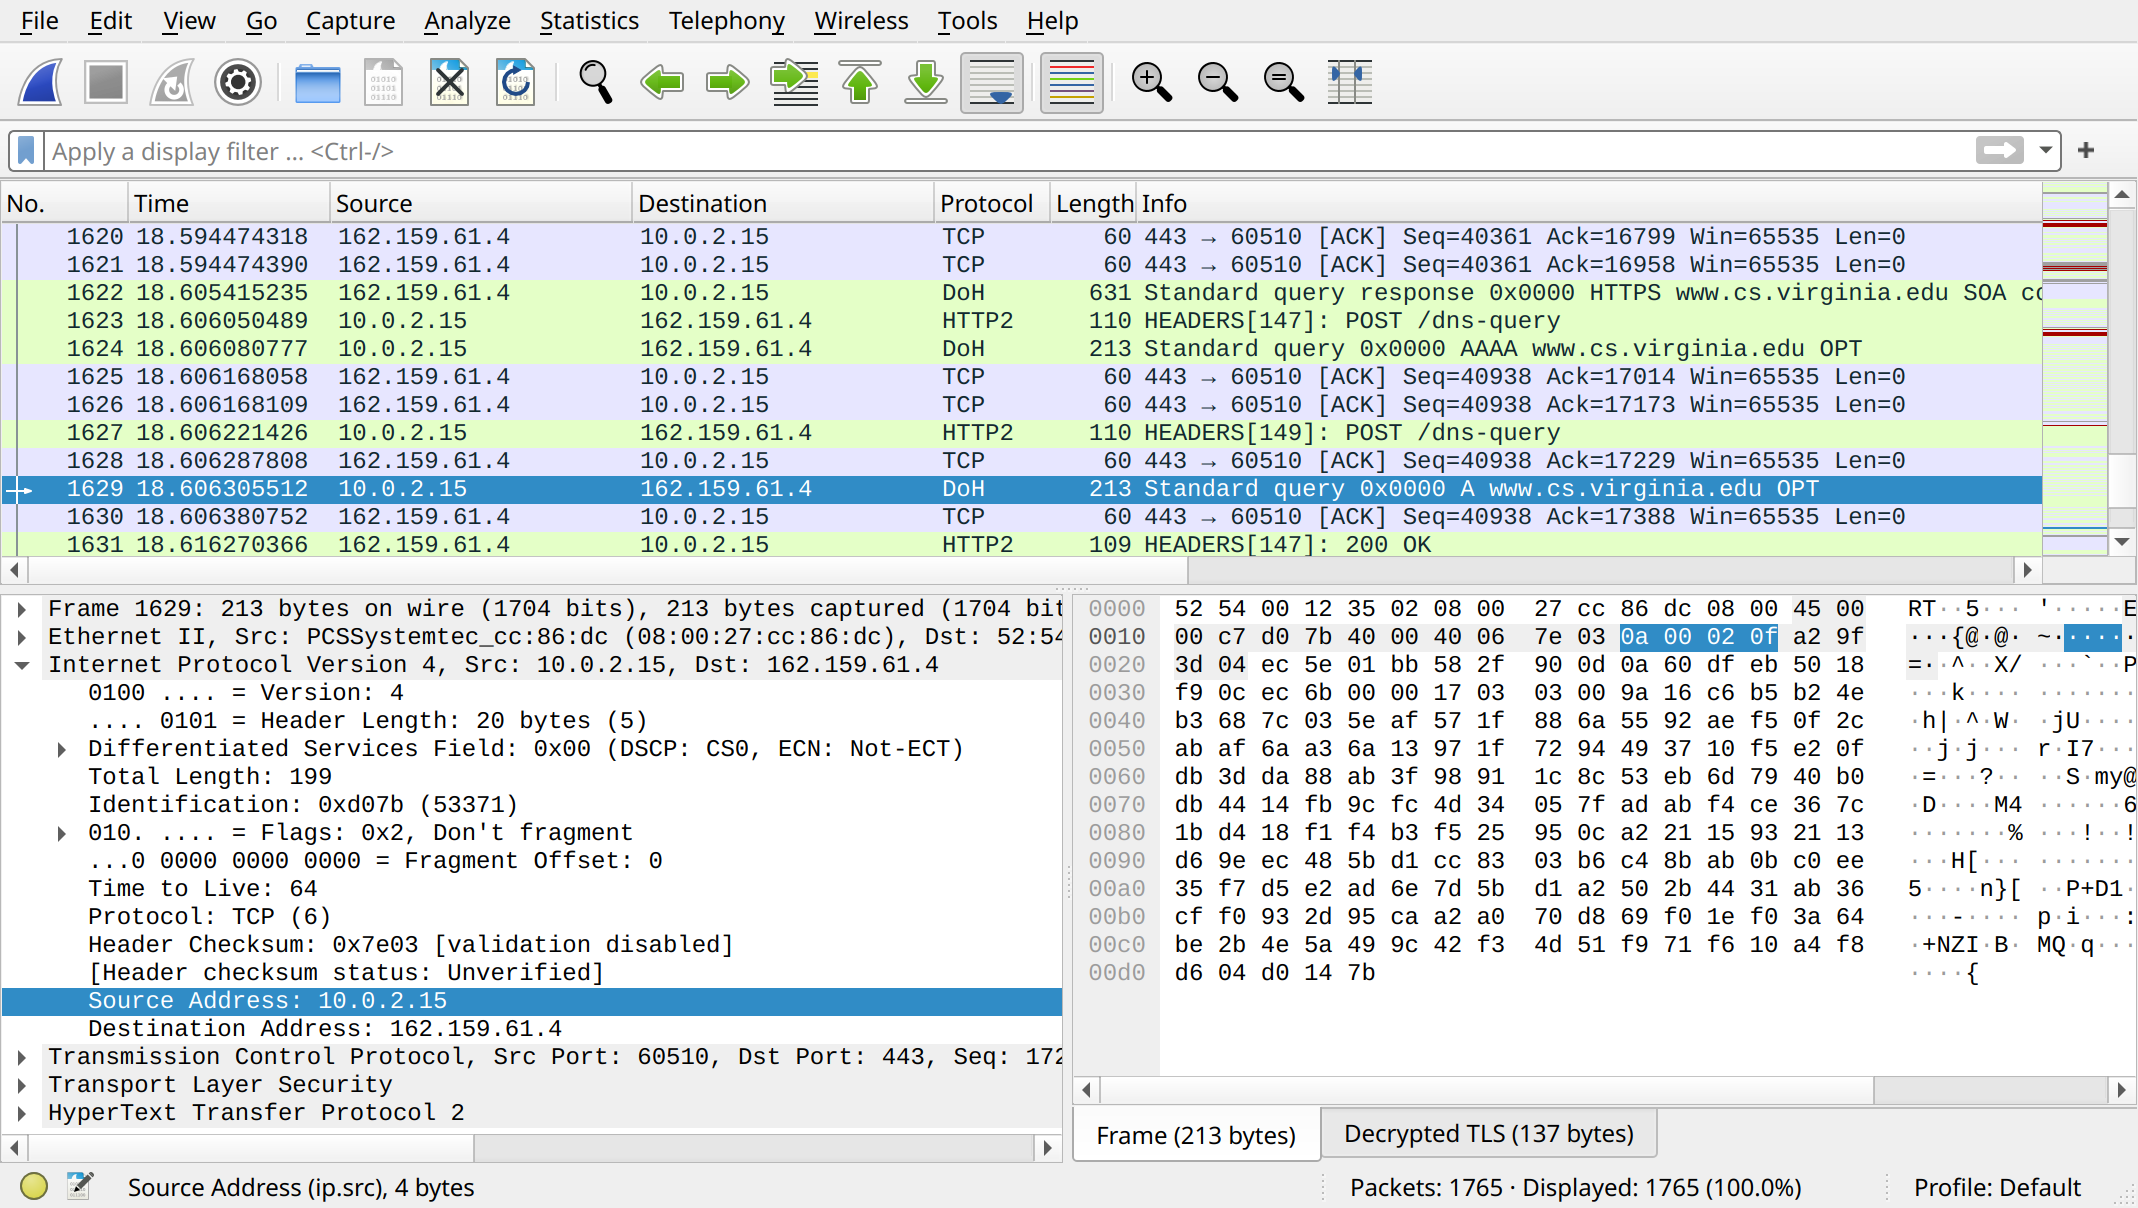
\includegraphics[width=\textwidth]{../intro/wireshark-example1.png}
};
\begin{visibleenv}<1>
    \node[text=red,overlay box] at (7.5, -2) {wireshark window};
\end{visibleenv}
\path (0, 0) rectangle (14.5, -7); % for bounding box
%\draw[overlay,help lines] (0, 0) grid (14, -8);
\begin{visibleenv}<3>
    \path[draw,red,very thick] (0, -1.2) rectangle (14.5, -4)
        node[midway,overlay box] { packet list };
    \path[draw,red,very thick] (0, -4) rectangle (7.25, -7.9)
        node[midway,overlay box] { packet details };
    \path[draw,red,very thick] (7.25, -4) rectangle (14.5, -7.9)
        node[midway,overlay box] { packet bytes };
\end{visibleenv}
\begin{visibleenv}<4>
    \path[draw,red,very thick] (0, -6.7) rectangle (7.2, -6.9);
    \path[draw,red,very thick] (10.93, -4.2) rectangle (12.1, -4.4);
    \path[draw,red,ultra thick] (7.2, -6.8) -- (10.93, -4.3)
        node[midway,above left,overlay box,align=left] {
            hilite in details \\
            shows corresponding bytes
        }
        node[midway,below right,overlay box,font=\fontsize{10}{11}\selectfont,text=black,align=left] {
            this case: \\
            \texttt{10} = \texttt{0x0a} \\
            \texttt{0} = \texttt{0x00} \\
            \texttt{2} = \texttt{0x02} \\
            \texttt{15} = \texttt{0x0f}
        };
\end{visibleenv}
\begin{visibleenv}<5>
    \path[draw,red,very thick] (6.3, -1.2) rectangle (7.15, -4);
    \node[overlay box,anchor=west] at (7.15, -3) (protocol) {`protocol'};
    \node[overlay box,font=\small,anchor=north west] at (protocol.south west) {
        the highest-layer protocol decoded
    };
\end{visibleenv}
\begin{visibleenv}<6-7>
    \begin{scope}
        \begin{pgfinterruptboundingbox}
    \tikzset{invclip/.style={clip,insert path={{[reset cm]
          (-16383.99999pt,-16383.99999pt) rectangle (16383.99999pt,16383.99999pt)
      }}}}
        \path[invclip] (6.3, -3.2) rectangle (7.15, -3.4);
        \end{pgfinterruptboundingbox}

        \fill[overlay,white,fill opacity=0.8] (0, 0) rectangle (14.5, -1.2);
        \fill[white,fill opacity=0.8] (0, -1.2) rectangle (14.5, -4);
        \fill[white,fill opacity=0.8] (7.25, -4) rectangle (14.5, -7.9);
    \end{scope}
    \path[draw,red,very thick] (0, -4) rectangle (7.25, -7.9);
    \tikzset{
        protomark/.style={Latex-,blue,thick},
        protomark brace/.style={blue,thick,decorate,decoration={brace}},
        protomark label/.style={blue,fill=white,fill opacity=0.9},
    }
    \draw[protomark] (7.25, -4.3) -- ++(1, 0) node[right,protomark label] {ethernet};
    \draw[protomark brace] (7.3, -4.5) -- (7.3, -7.1);
        \draw[protomark] (7.4, -5.8) -- ++ (0.75, .6) node[right, protomark label] {
                IPv4 (internet protocol version 4)
        };
    \draw[protomark] (7.25, -7.2) -- ++(1, 1) node[right,protomark label] {
        TCP ({\fontsize{10}{11}\selectfont transmission control protocol})
    };
    \draw[protomark] (7.25, -7.325) -- ++(1, .5) node[right,protomark label] {
        TLS ({\fontsize{10}{11}\selectfont transport layer security})
    };
    \draw[protomark] (7.25, -7.45) -- ++(1, -.2) node[right,protomark label] {
        HTTP/2 ({\fontsize{10}{11}\selectfont hypertext transfer protocol 2})
    };
\end{visibleenv}
\begin{visibleenv}<7>
    \draw[red, very thick] (6.3, -3.2) rectangle (7.15, -3.4);
    \draw[red,Latex-,very thick] (7.15, -3.3) -- ++(1, 0) node[right,align=left,overlay box] {
        DoH is not \\one of these!
    };
\end{visibleenv}
\end{tikzpicture}
\end{frame}

\begin{frame}{}
\begin{tikzpicture}
\tikzset{
    overlay box/.style={fill=white,fill opacity=0.9}
}
\node[overlay,anchor=north west,inner sep=0mm] (base) at (0, 0) {
    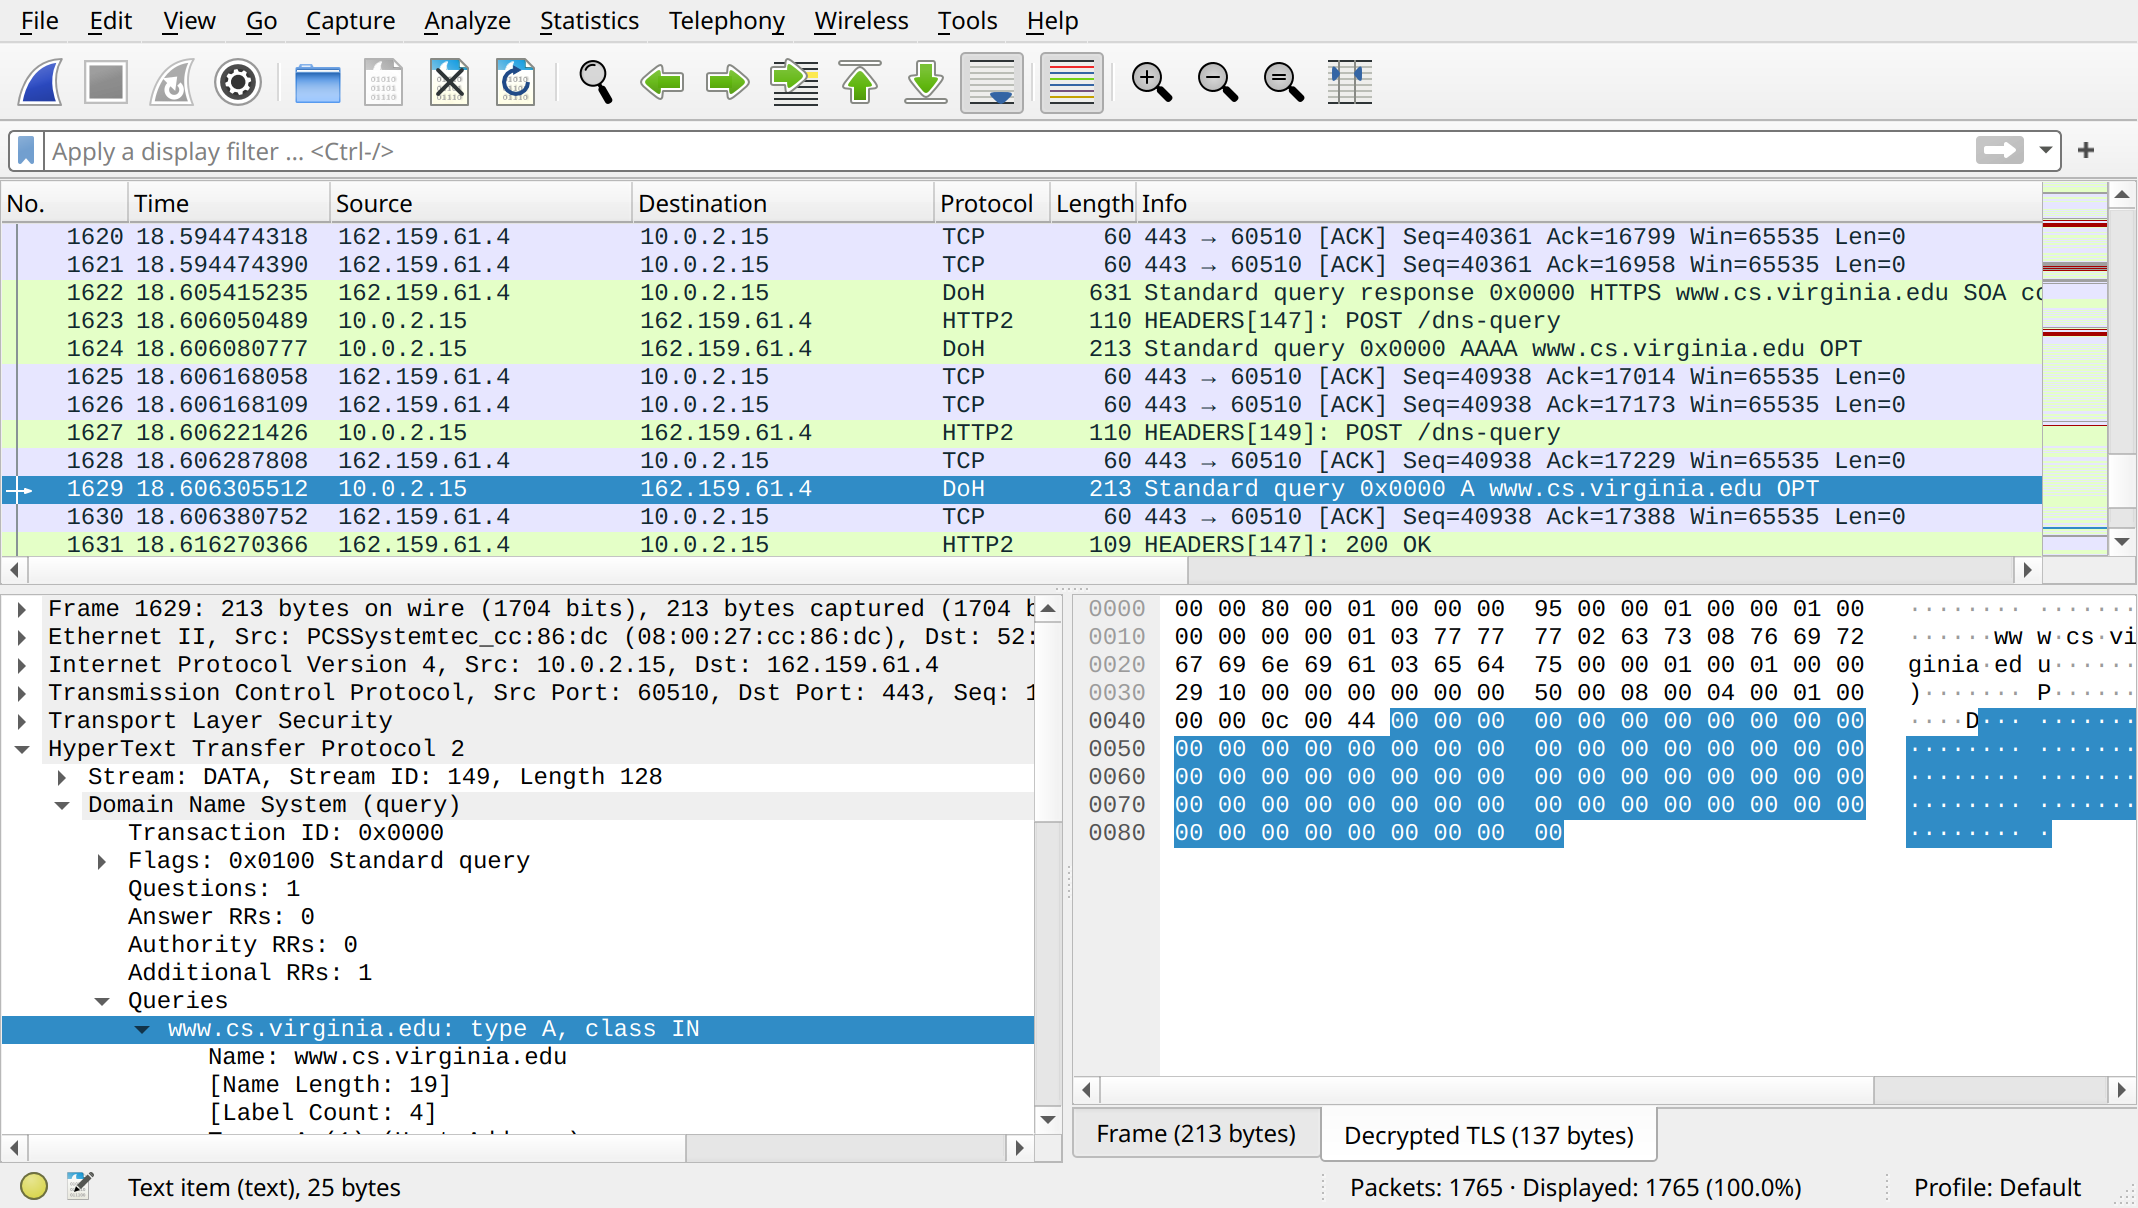
\includegraphics[width=\textwidth]{../intro/wireshark-doh-zoom.png}
};
\path (0, 0) rectangle (14.5, -7); % for bounding box
%\draw[overlay,help lines] (0, 0) grid (14, -8);
    \begin{scope}
        \begin{pgfinterruptboundingbox}
    \tikzset{invclip/.style={clip,insert path={{[reset cm]
          (-16383.99999pt,-16383.99999pt) rectangle (16383.99999pt,16383.99999pt)
      }}}}
        \path[invclip] (6.3, -3.2) rectangle (7.15, -3.4);
        \end{pgfinterruptboundingbox}

        \fill[overlay,white,fill opacity=0.8] (0, 0) rectangle (14.5, -1.2);
        \fill[white,fill opacity=0.8] (0, -1.2) rectangle (14.5, -4);
        \fill[white,fill opacity=0.8] (7.25, -4) rectangle (14.5, -7.9);
    \end{scope}
    \path[draw,red,very thick] (0, -4) rectangle (7.25, -7.9);
    \tikzset{
        protomark/.style={Latex-,blue,thick},
        protomark alt/.style={Latex-,violet,thick,dotted},
        protomark brace/.style={blue,thick,decorate,decoration={brace}},
        protomark brace alt/.style={violet,thick,decorate,decoration={brace}},
        protomark label/.style={blue,fill=white,fill opacity=0.9},
    }
    \draw[protomark] (7.25, -4.3) -- ++(1, .2) node[right,protomark label] {ethernet};
    \draw[protomark] (7.25, -4.5) -- ++ (1, -.2) node[right, protomark label] {
                IPv4 (internet protocol version 4)
        };
    \draw[protomark] (7.25, -4.6) -- ++(1, -.6) node[right,protomark label] {
        TCP ({\fontsize{10}{11}\selectfont transmission control protocol})
    };
    \draw[protomark] (7.25, -4.8) -- ++(1, -1) node[right,protomark label] {
        TLS ({\fontsize{10}{11}\selectfont transport layer security})
    };
    \draw[protomark brace] (7.3, -5) -- (7.3, -7.9);
        \draw[protomark] (7.4, -6.5) -- ++ (0.75, 0) node[right, protomark label] {
            HTTP/2 ({\fontsize{10}{11}\selectfont hypertext transfer protocol 2})
        };
    \draw[protomark brace alt] (7.5, -5.5) -- (7.5, -7.9);
        \draw[protomark alt] (7.6, -6.85) -- ++ (0.75, -.5) node[right, protomark label] {
            DNS (domain name system)
        };
    \draw[red, very thick] (6.3, -3.2) rectangle (7.15, -3.4);
    \draw[red,Latex-,very thick] (7.15, -3.3) -- ++(1, 0) node[right,align=left,overlay box] {
        DoH = DNS over HTTPS
    };
\end{tikzpicture}
\end{frame}

\begin{frame}[fragile]{}
\providecommand{\doHilite}[6]{
    %\doHilite{Y offset start protocol list}{Y offset end protocol list}
    %         {X offset corner data}{Y offset corner data}
    %         {X offset other corner data}{Y offset other corner data}
    \path[draw,red,very thick] (0, -3.95 - #1 * 0.206) rectangle (7.25, -3.95 - #2 * 0.206);
    \path[draw,red,very thick] (7.95 + #3, -4.2059 - #4 * 0.2059) -- (7.95 + #3, -3.95 - #4 * 0.2059)
            -- (12.8, -3.95 - #4 * 0.2059)
            |- (7.95 + #5, -4 - #6 * 0.2059) 
            |- (7.95, -4 - #6 * 0.2059 - .2059) |- cycle;
}
\providecommand{\doHiliteOneDataLine}[6]{
    %\doHilite{Y offset start protocol list}{Y offset end protocol list}
    %         {X offset corner data}{Y offset corner data}
    %         {X offset other corner data}{Y offset other corner data}

    \path[draw,red,very thick] (0, -3.95 - #1 * 0.207) rectangle (7.25, -4 - #2 * 0.207);
    \path[draw,red,very thick] (7.95 + #3, -4.207 - #4 * 0.207) -- (7.95 + #3, -4 - #4 * 0.207)
            %-- (12.8, -4 - #4 * 0.207)
            |- (7.95 + #5, -4 - #6 * 0.207) 
            |- (7.95, -4 - #6 * 0.207 - .207) |- cycle;
}
\begin{tikzpicture}
\tikzset{
    overlay box/.style={fill=white,fill opacity=0.9},
}
\node[overlay,anchor=north west,inner sep=0mm] (base) at (0, 0) {%
\only<1-2>{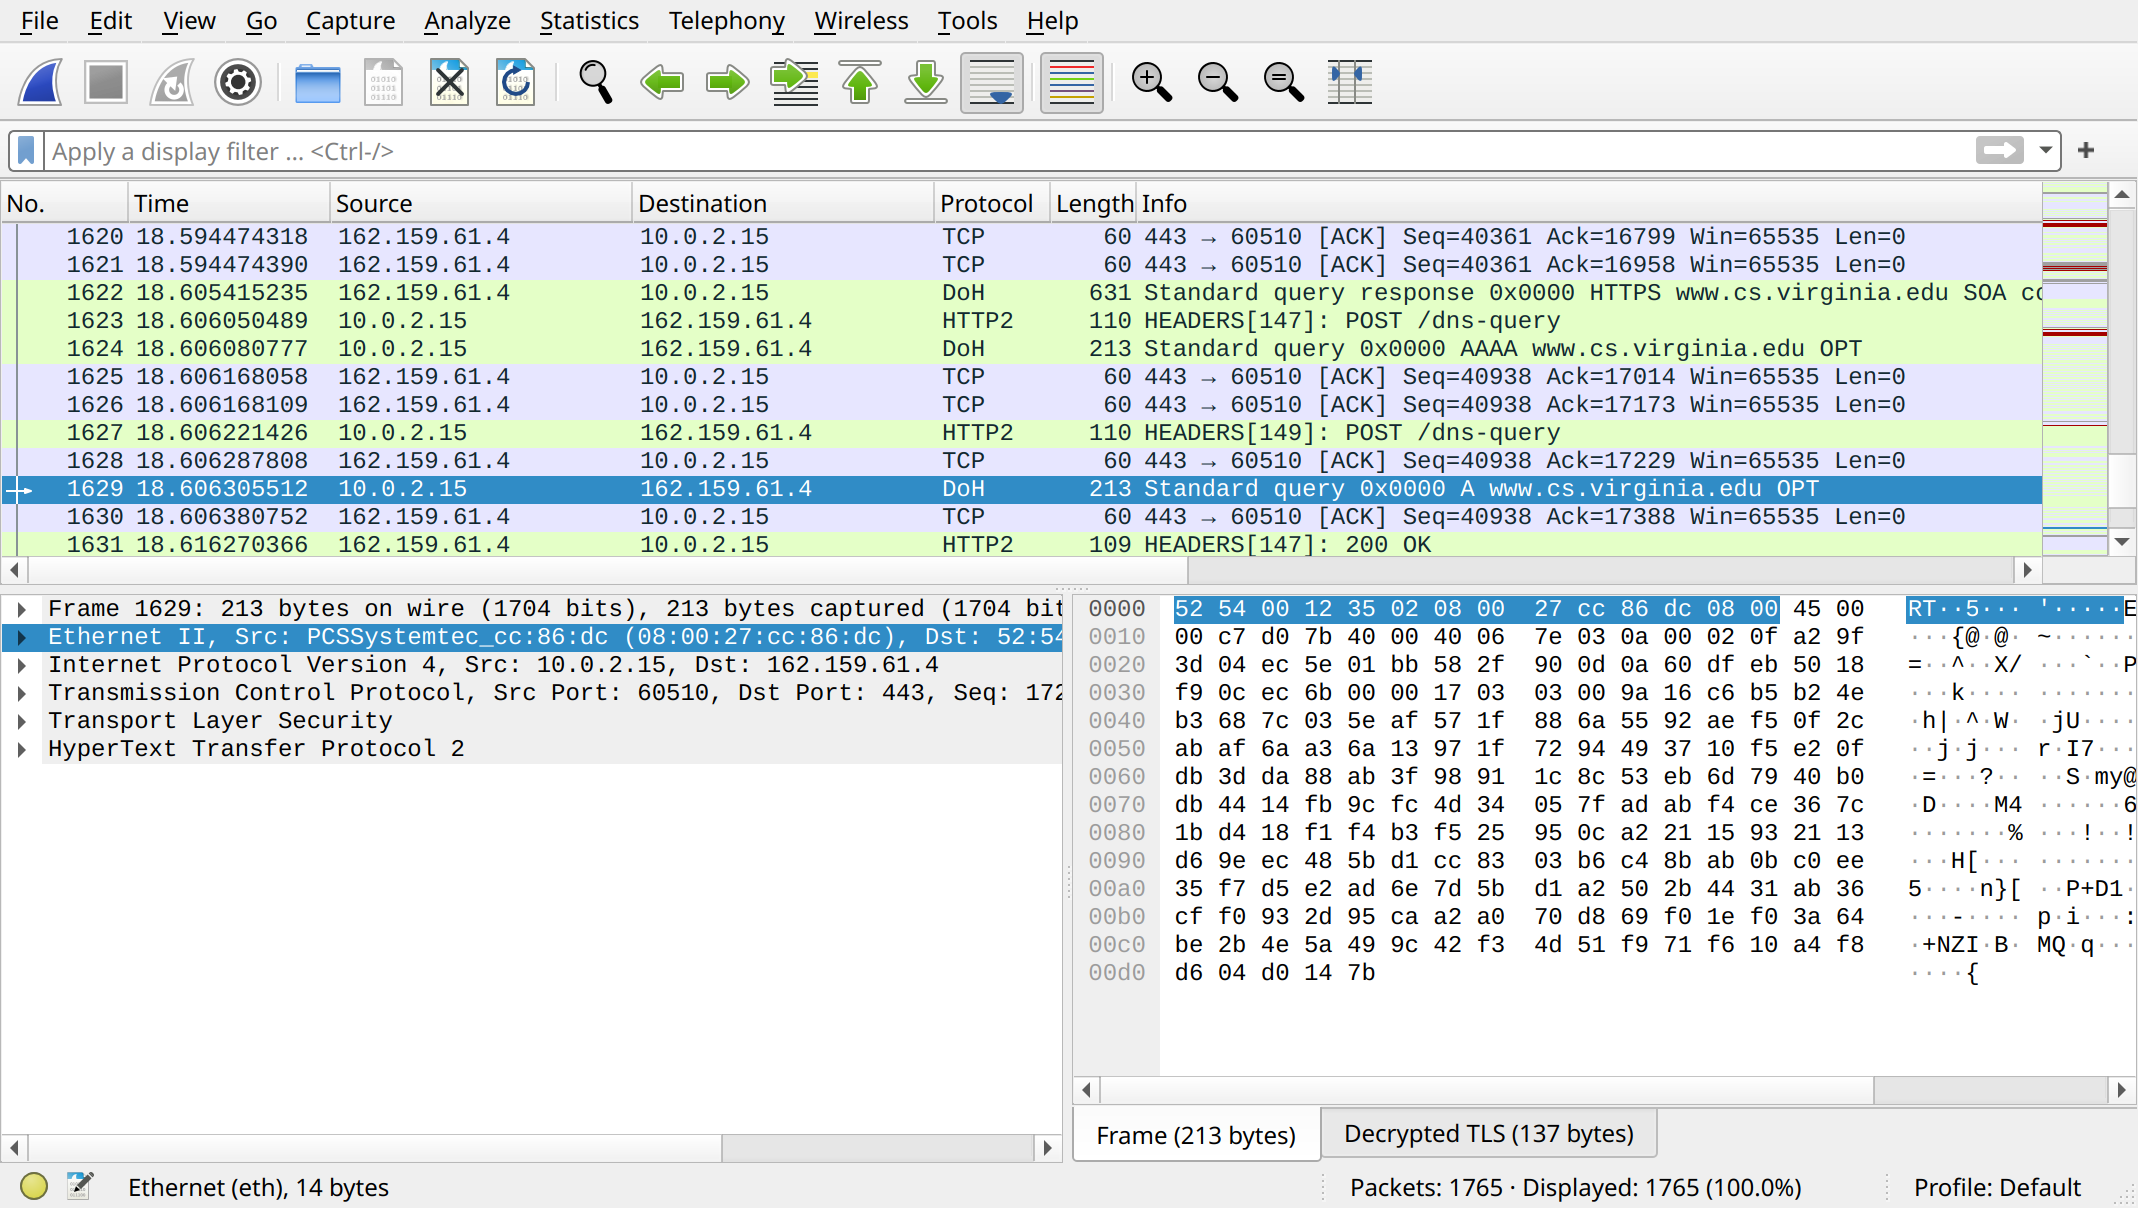
\includegraphics[width=\textwidth]{../intro/wireshark-hi-ethernet.png}}%
\only<3-4>{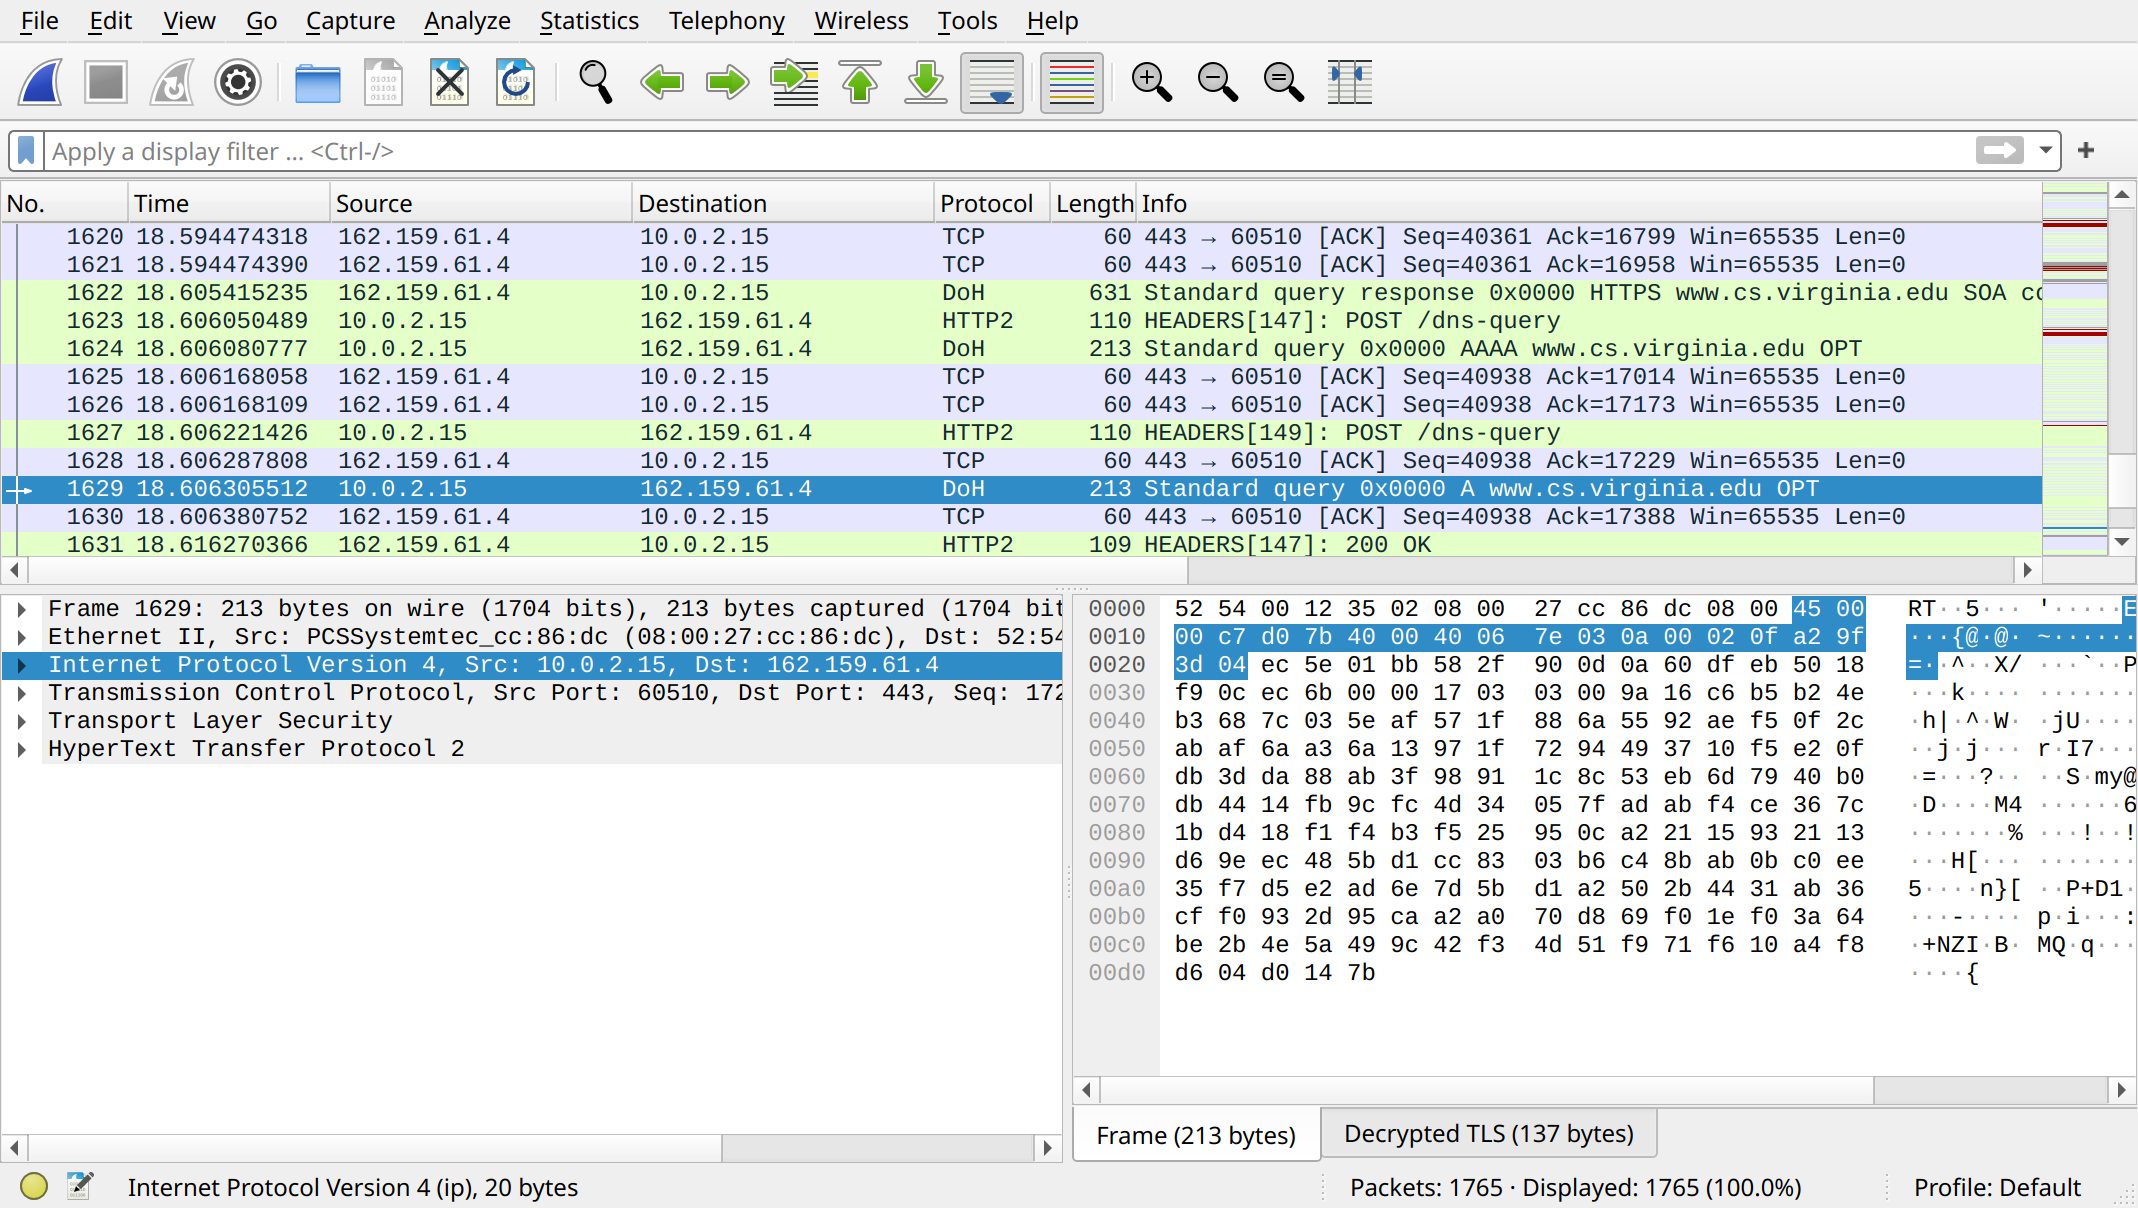
\includegraphics[width=\textwidth]{../intro/wireshark-hi-ipv4.png}}%
\only<5-6>{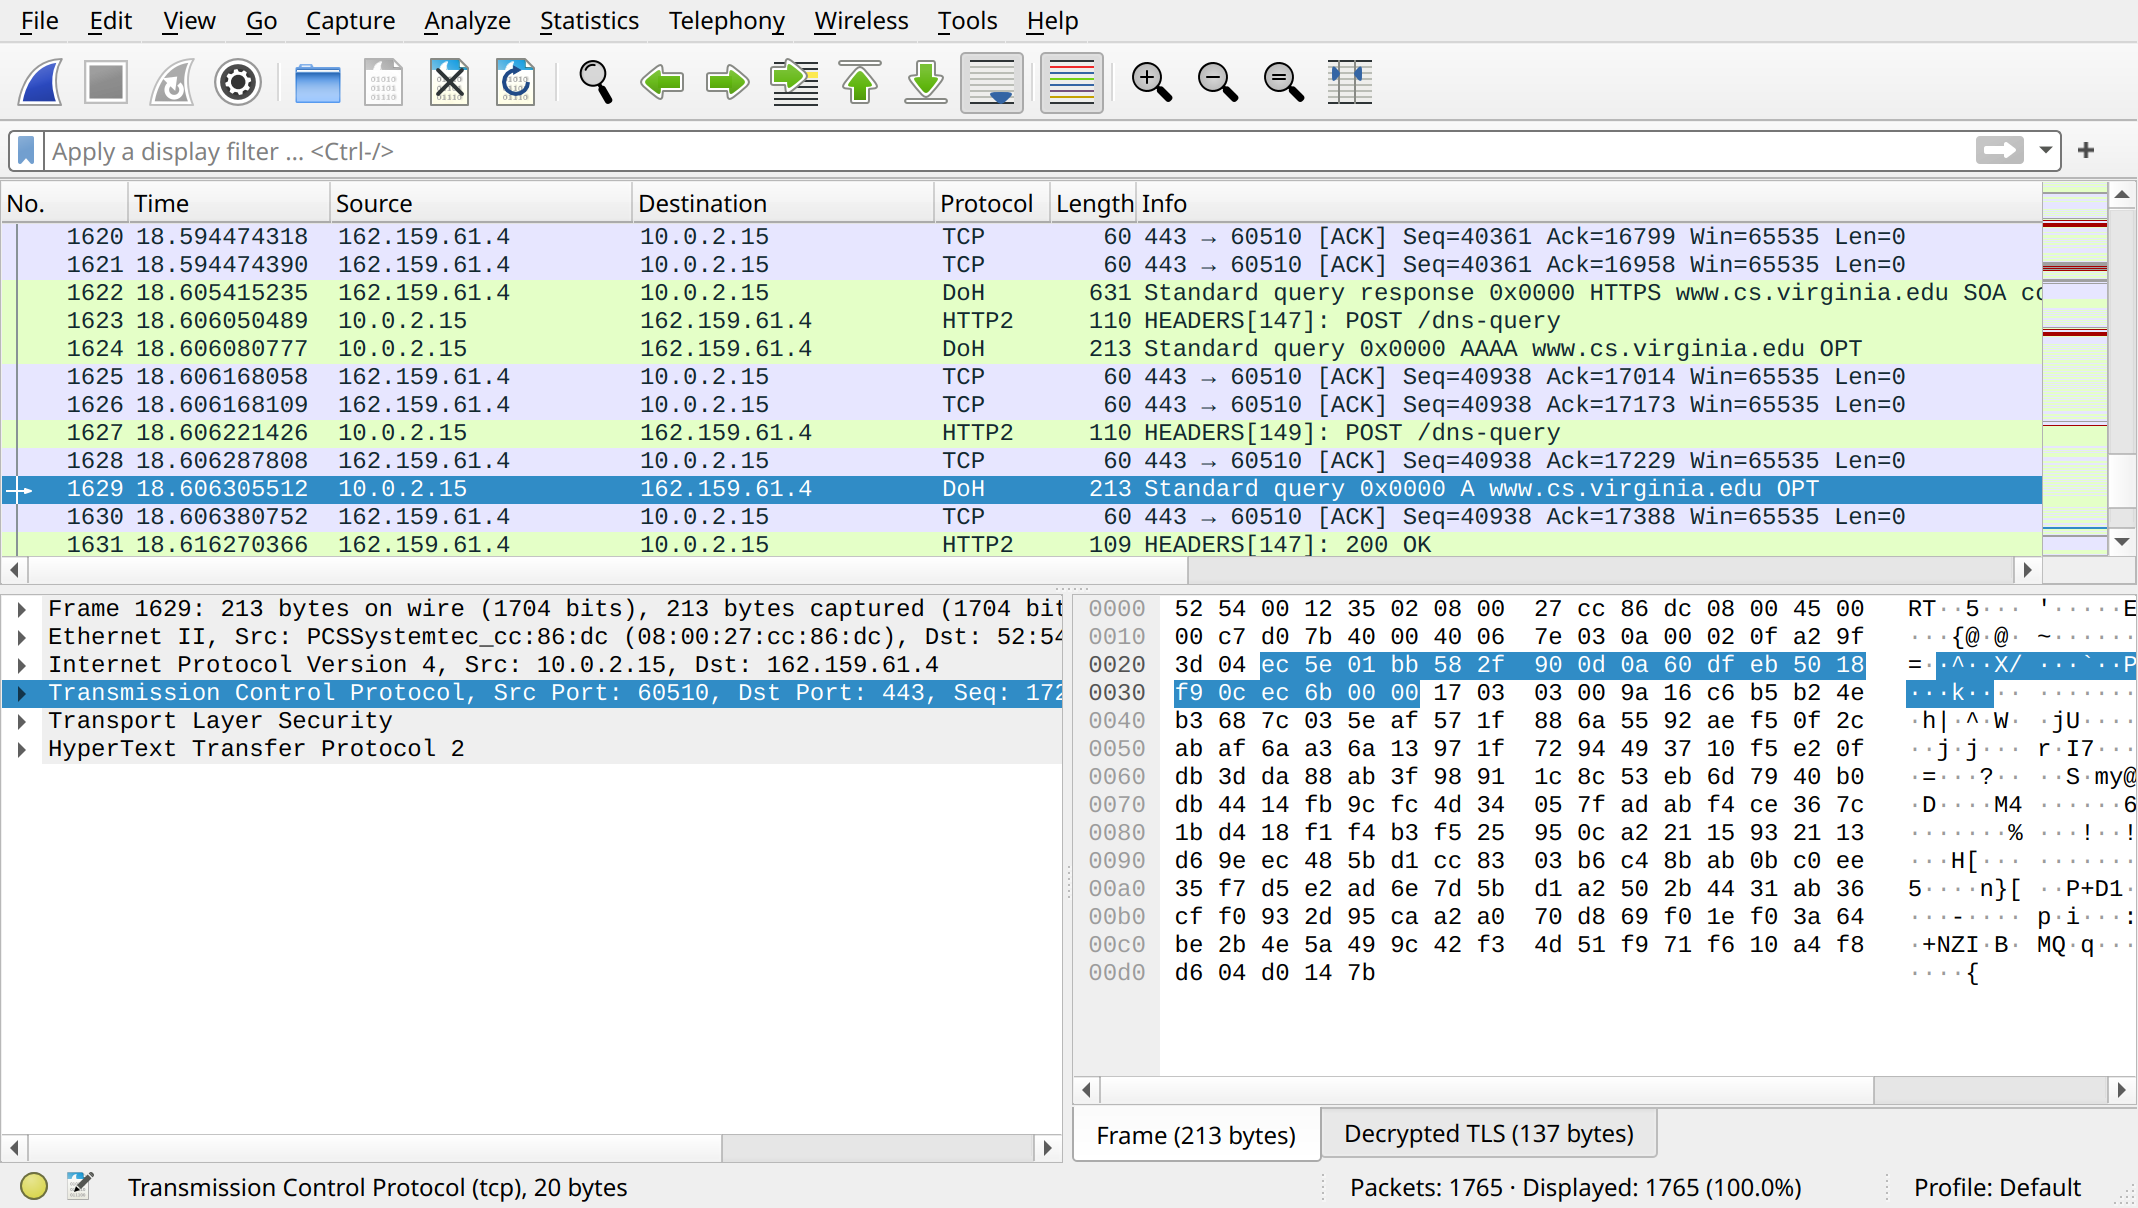
\includegraphics[width=\textwidth]{../intro/wireshark-hi-tcp.png}}%
\only<7-8>{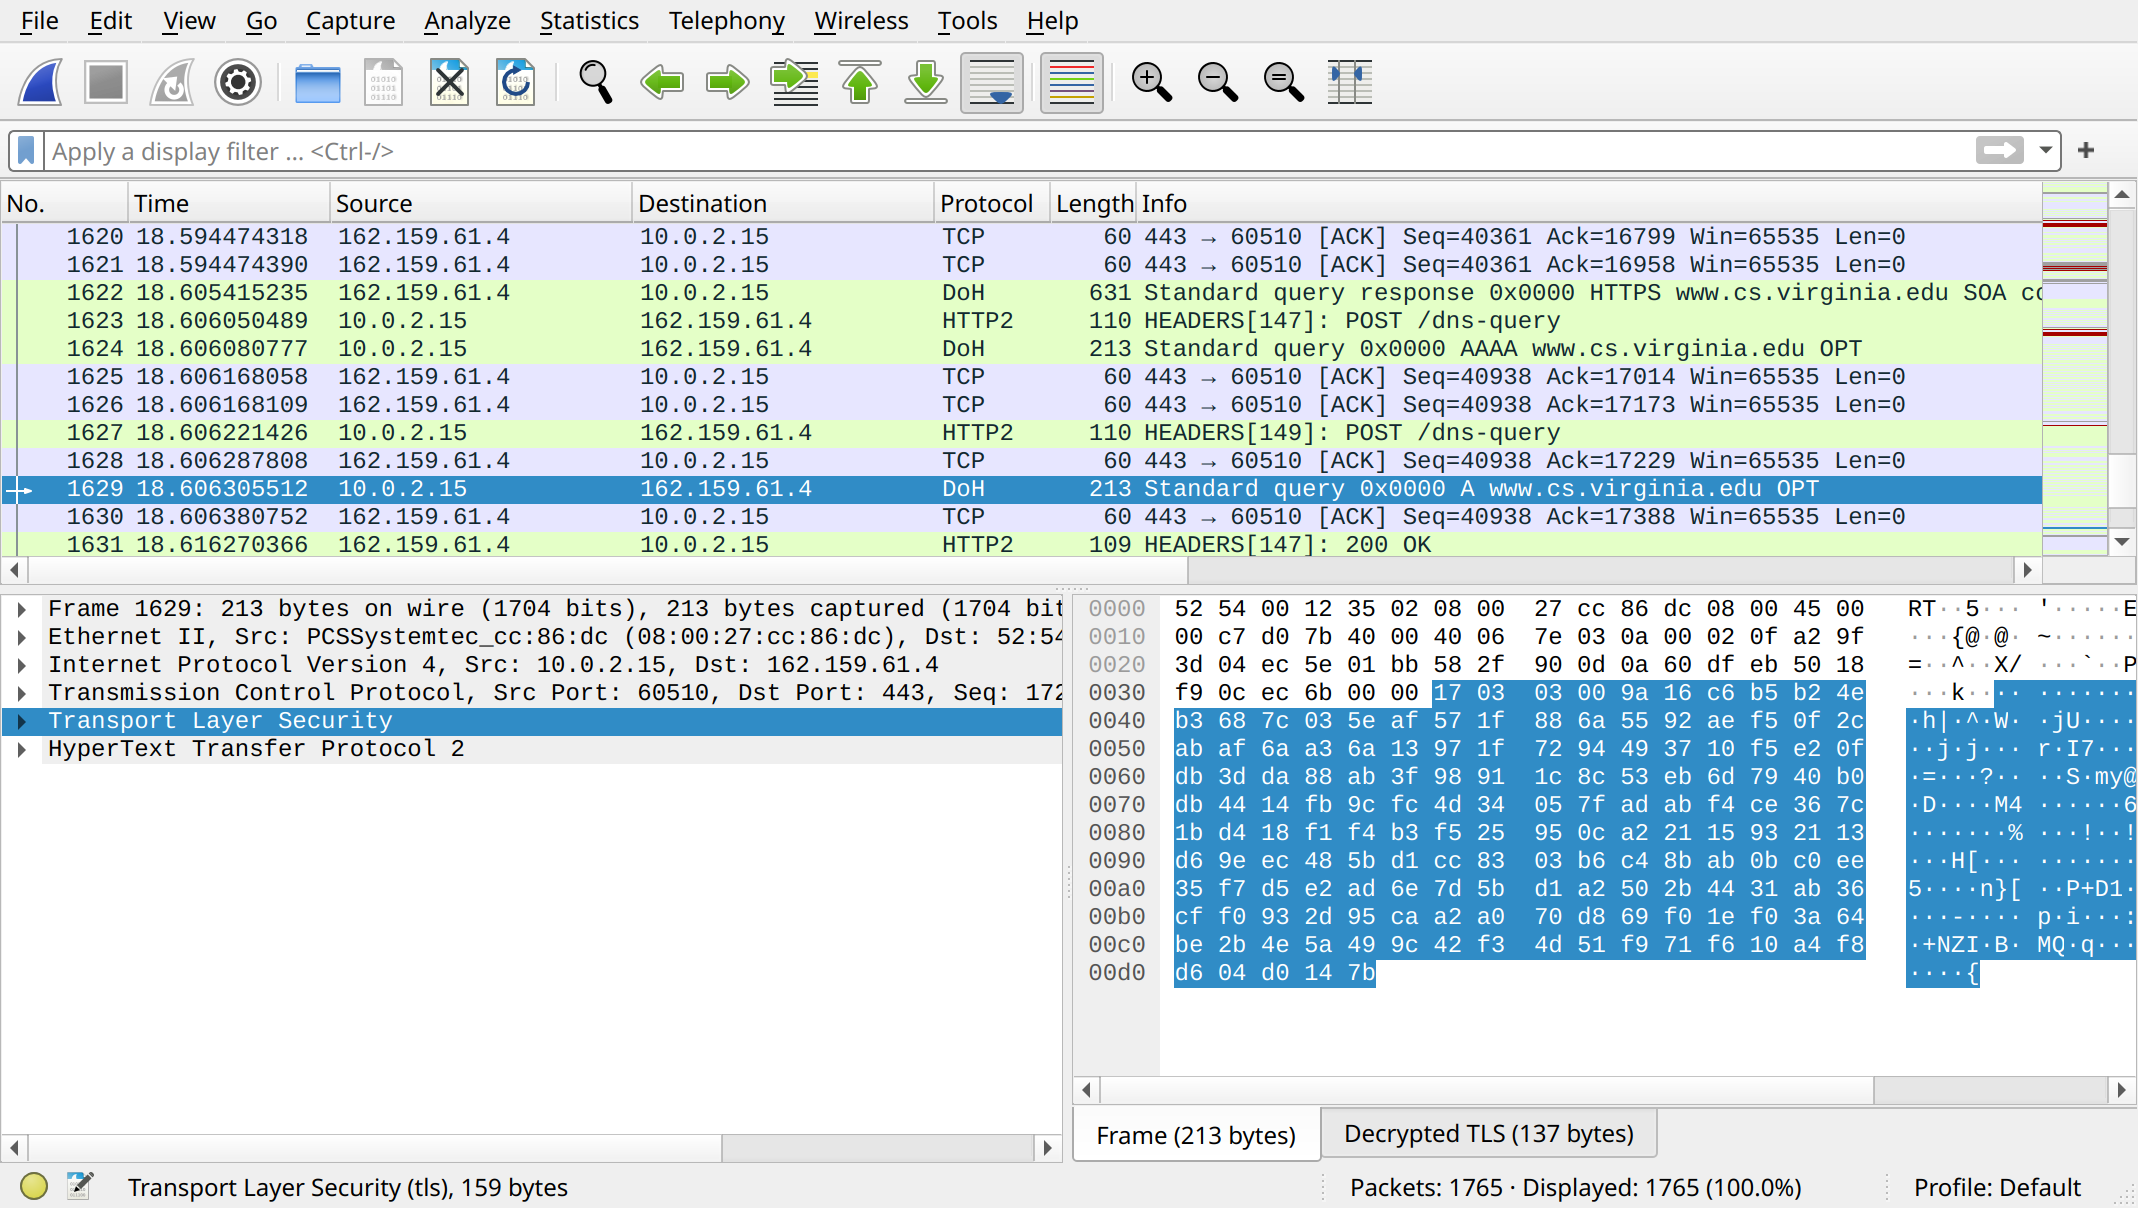
\includegraphics[width=\textwidth]{../intro/wireshark-hi-tls.png}}%
\only<9-11>{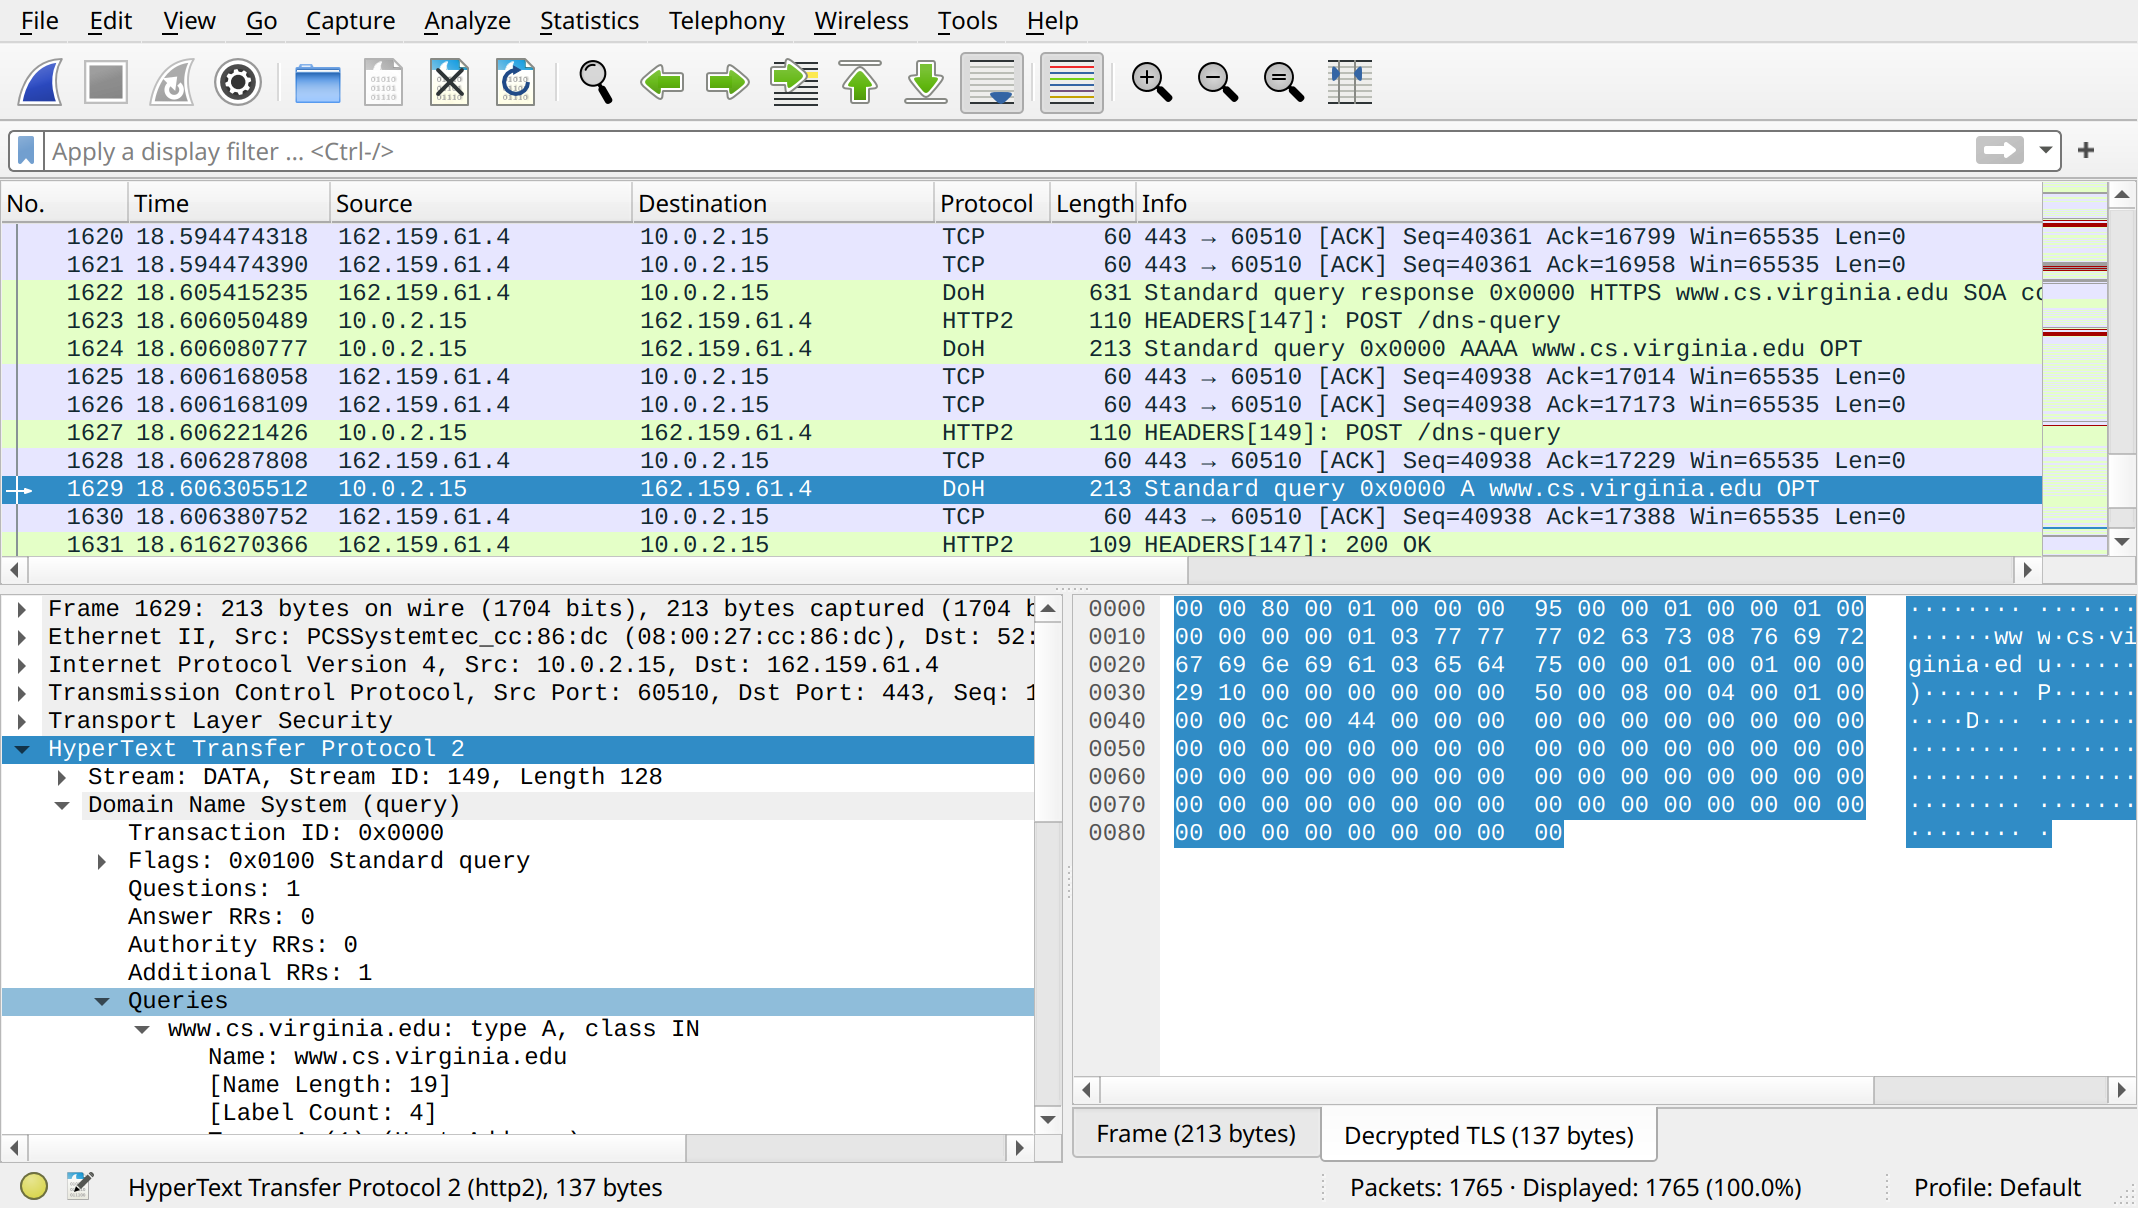
\includegraphics[width=\textwidth]{../intro/wireshark-hi-http.png}}%
\only<12-13>{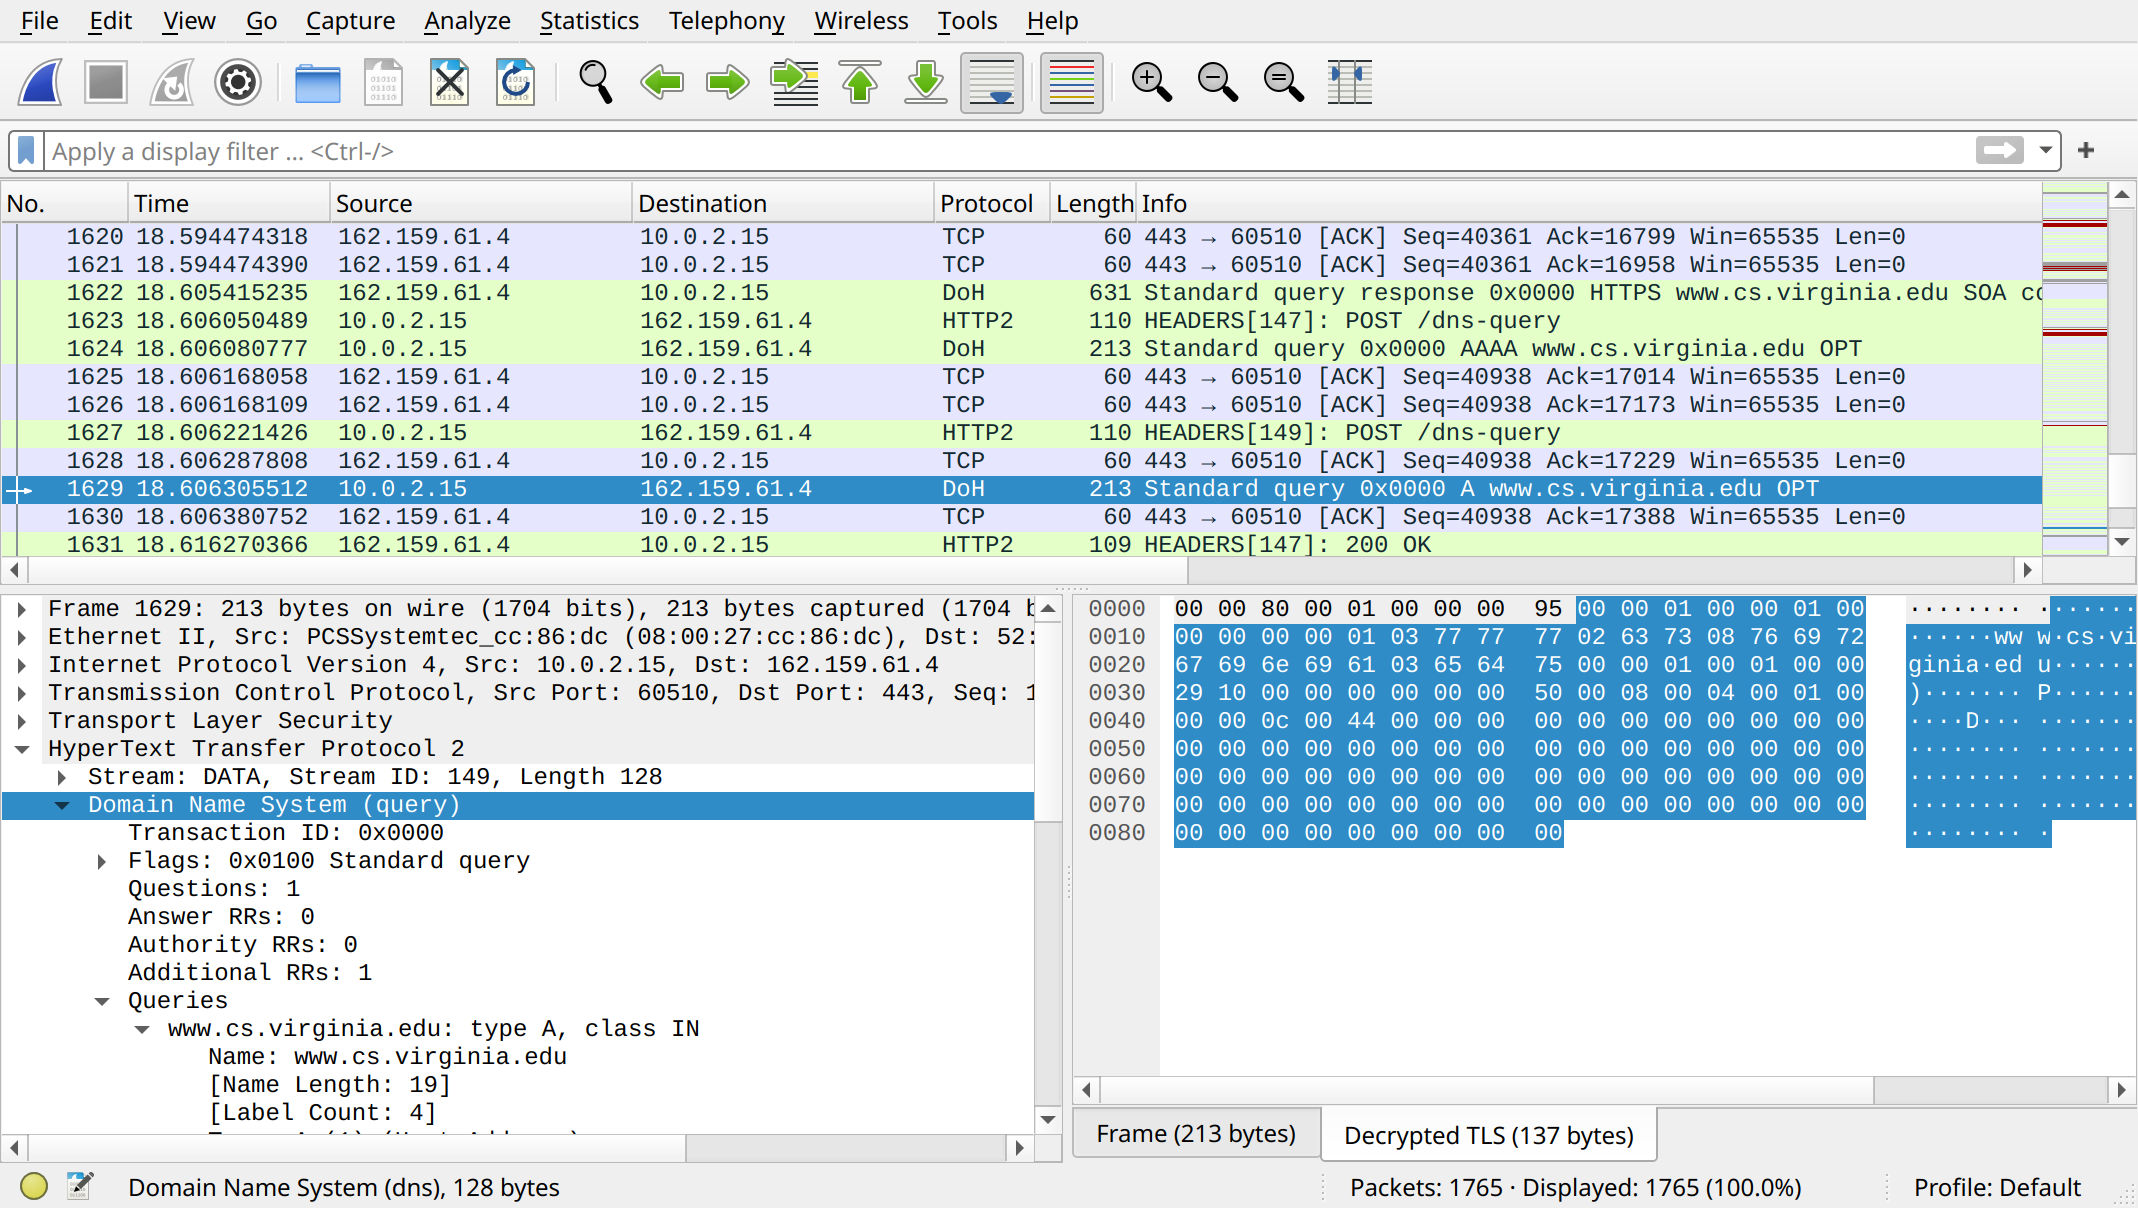
\includegraphics[width=\textwidth]{../intro/wireshark-hi-dns-in-tls.png}}%
};
%\draw[overlay,help lines] (0, 0) grid (14, -8);
\path (0, 0) rectangle (14.5, -7); % for bounding box

\begin{visibleenv}<1> % ethernet
    \doHiliteOneDataLine{1}{2}{0}{0}{4.2}{0}
\end{visibleenv}
\begin{visibleenv}<3> % IP
    \doHilite{2}{3}{4.2}{0}{0.5}{2}
\end{visibleenv}
\begin{visibleenv}<5> % TCP
    \doHilite{3}{4}{0.5}{2}{1.7}{3}
\end{visibleenv}
\begin{visibleenv}<7> % TLS
    \doHilite{4}{5}{1.7}{3}{1.4}{12}
\end{visibleenv}
\begin{visibleenv}<9> % HTTP, decrypted TLS
    \path[draw,red,very thick] (8.9, -7.5) rectangle (11.3, -7.9);
    \node[align=left,overlay box,anchor=south] at (10.4, -7.5) {
        setup step: got Firefox to output \\
        cryptographic keys ({\fontsize{10}{11}\selectfont using \tt SSLKEYLOGFILE})
    };
\end{visibleenv}
\begin{visibleenv}<10> % HTTP
    \doHilite{5}{6}{0}{0}{2.69}{8}
\end{visibleenv}
\begin{visibleenv}<12> % DNS
    \doHilite{7}{8}{2.7}{0}{2.69}{8}
\end{visibleenv}
\end{tikzpicture}
\end{frame}

% FIXME: show multiple related packets --- emphasize filter window
\begin{frame}{}
\begin{tikzpicture}
\tikzset{
    overlay box/.style={fill=white,fill opacity=0.9}
}
\node[overlay,anchor=north west,inner sep=0mm] (base) at (0, 0) {
    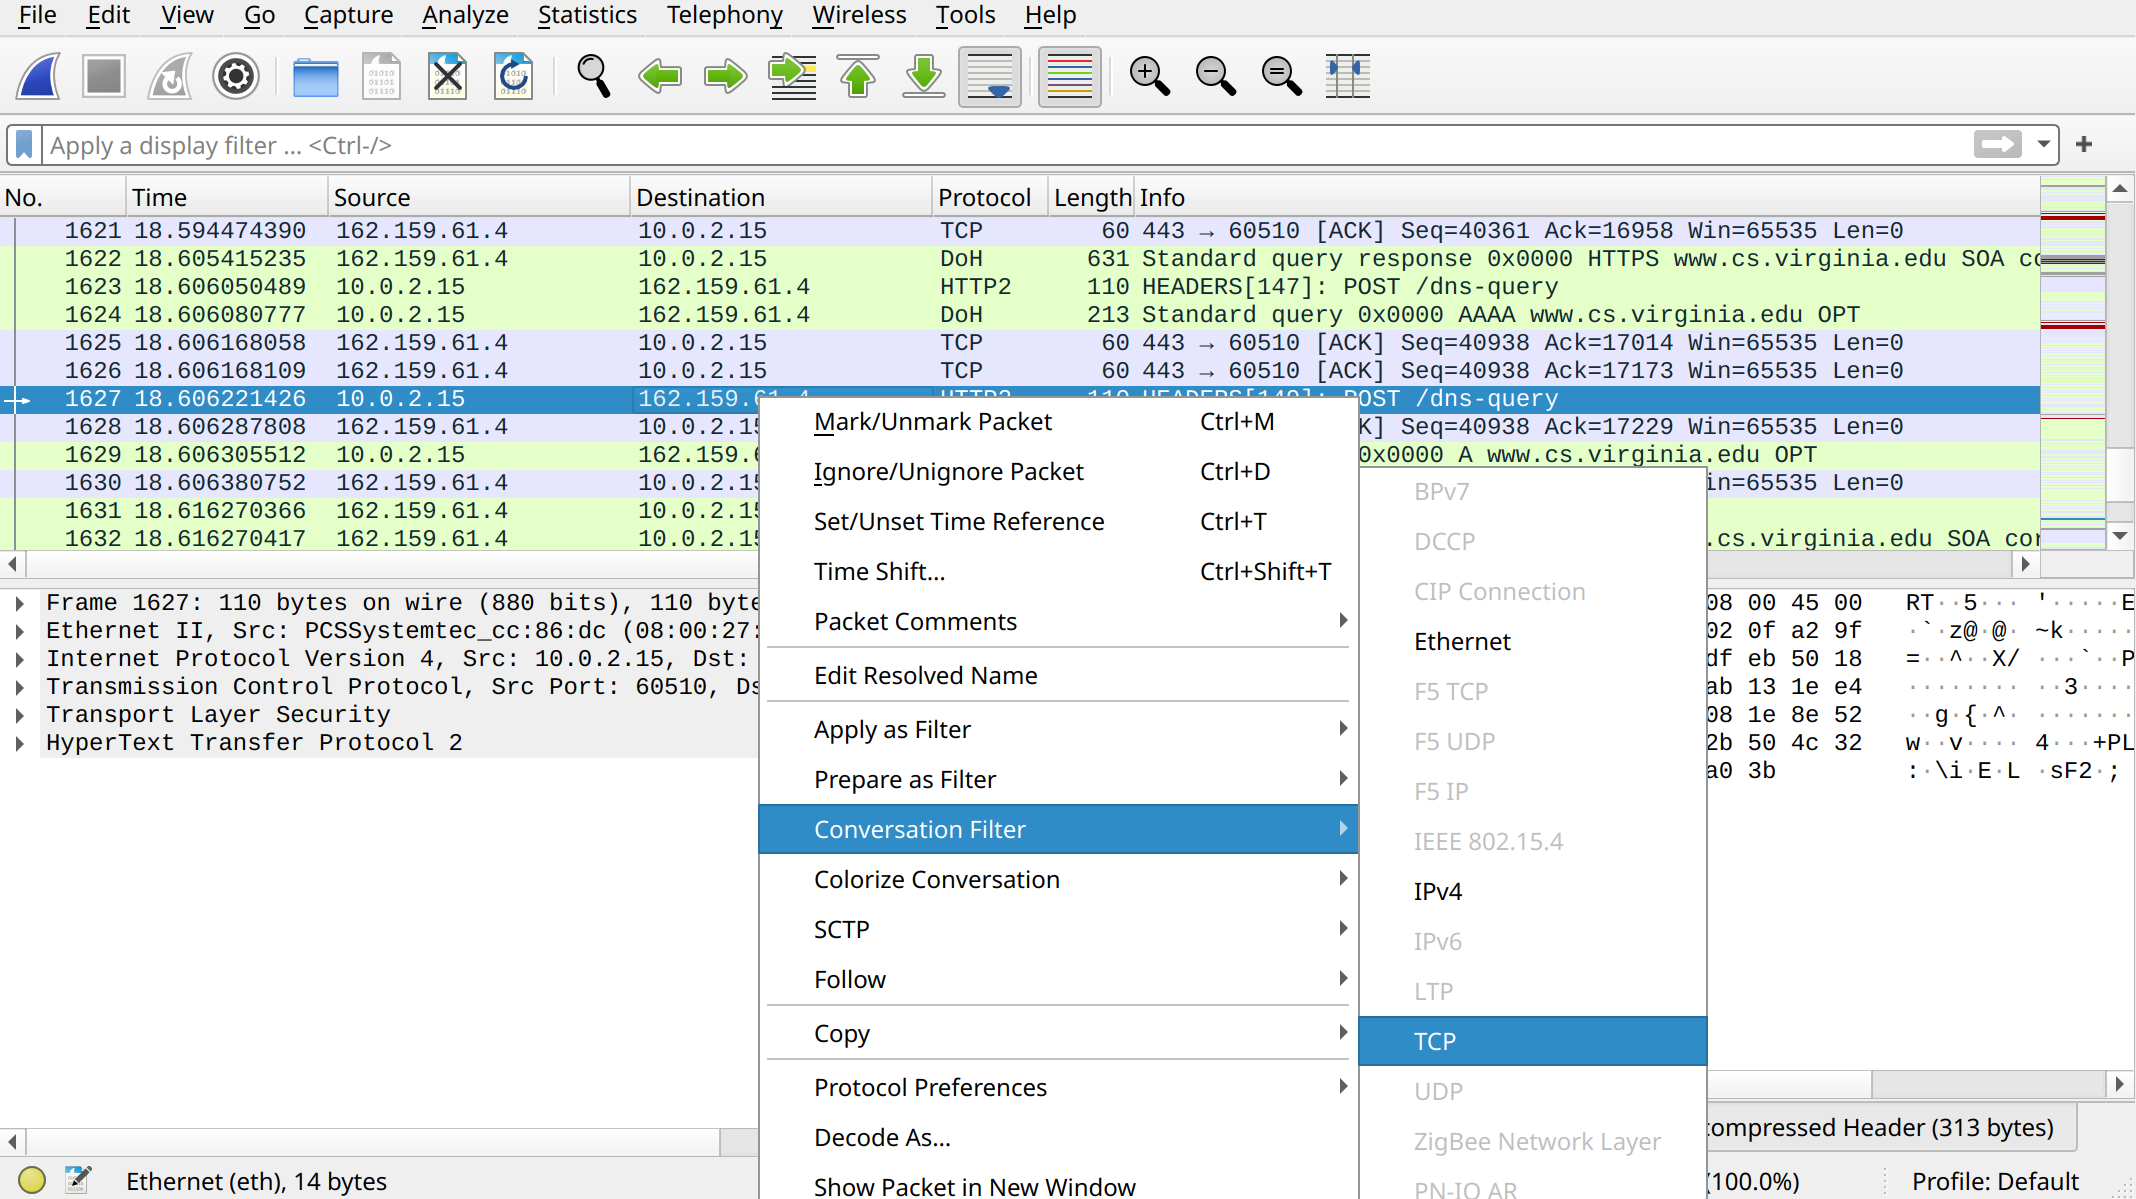
\includegraphics[width=\textwidth]{../intro/wireshark-menu-tcp-filter.png}
};
\path (0, 0) rectangle (14.5, -7); % for bounding box
\end{tikzpicture}
\end{frame}

\begin{frame}{}
\begin{tikzpicture}
\tikzset{
    overlay box/.style={fill=white,fill opacity=0.9}
}
\node[overlay,anchor=north west,inner sep=0mm] (base) at (0, 0) {
    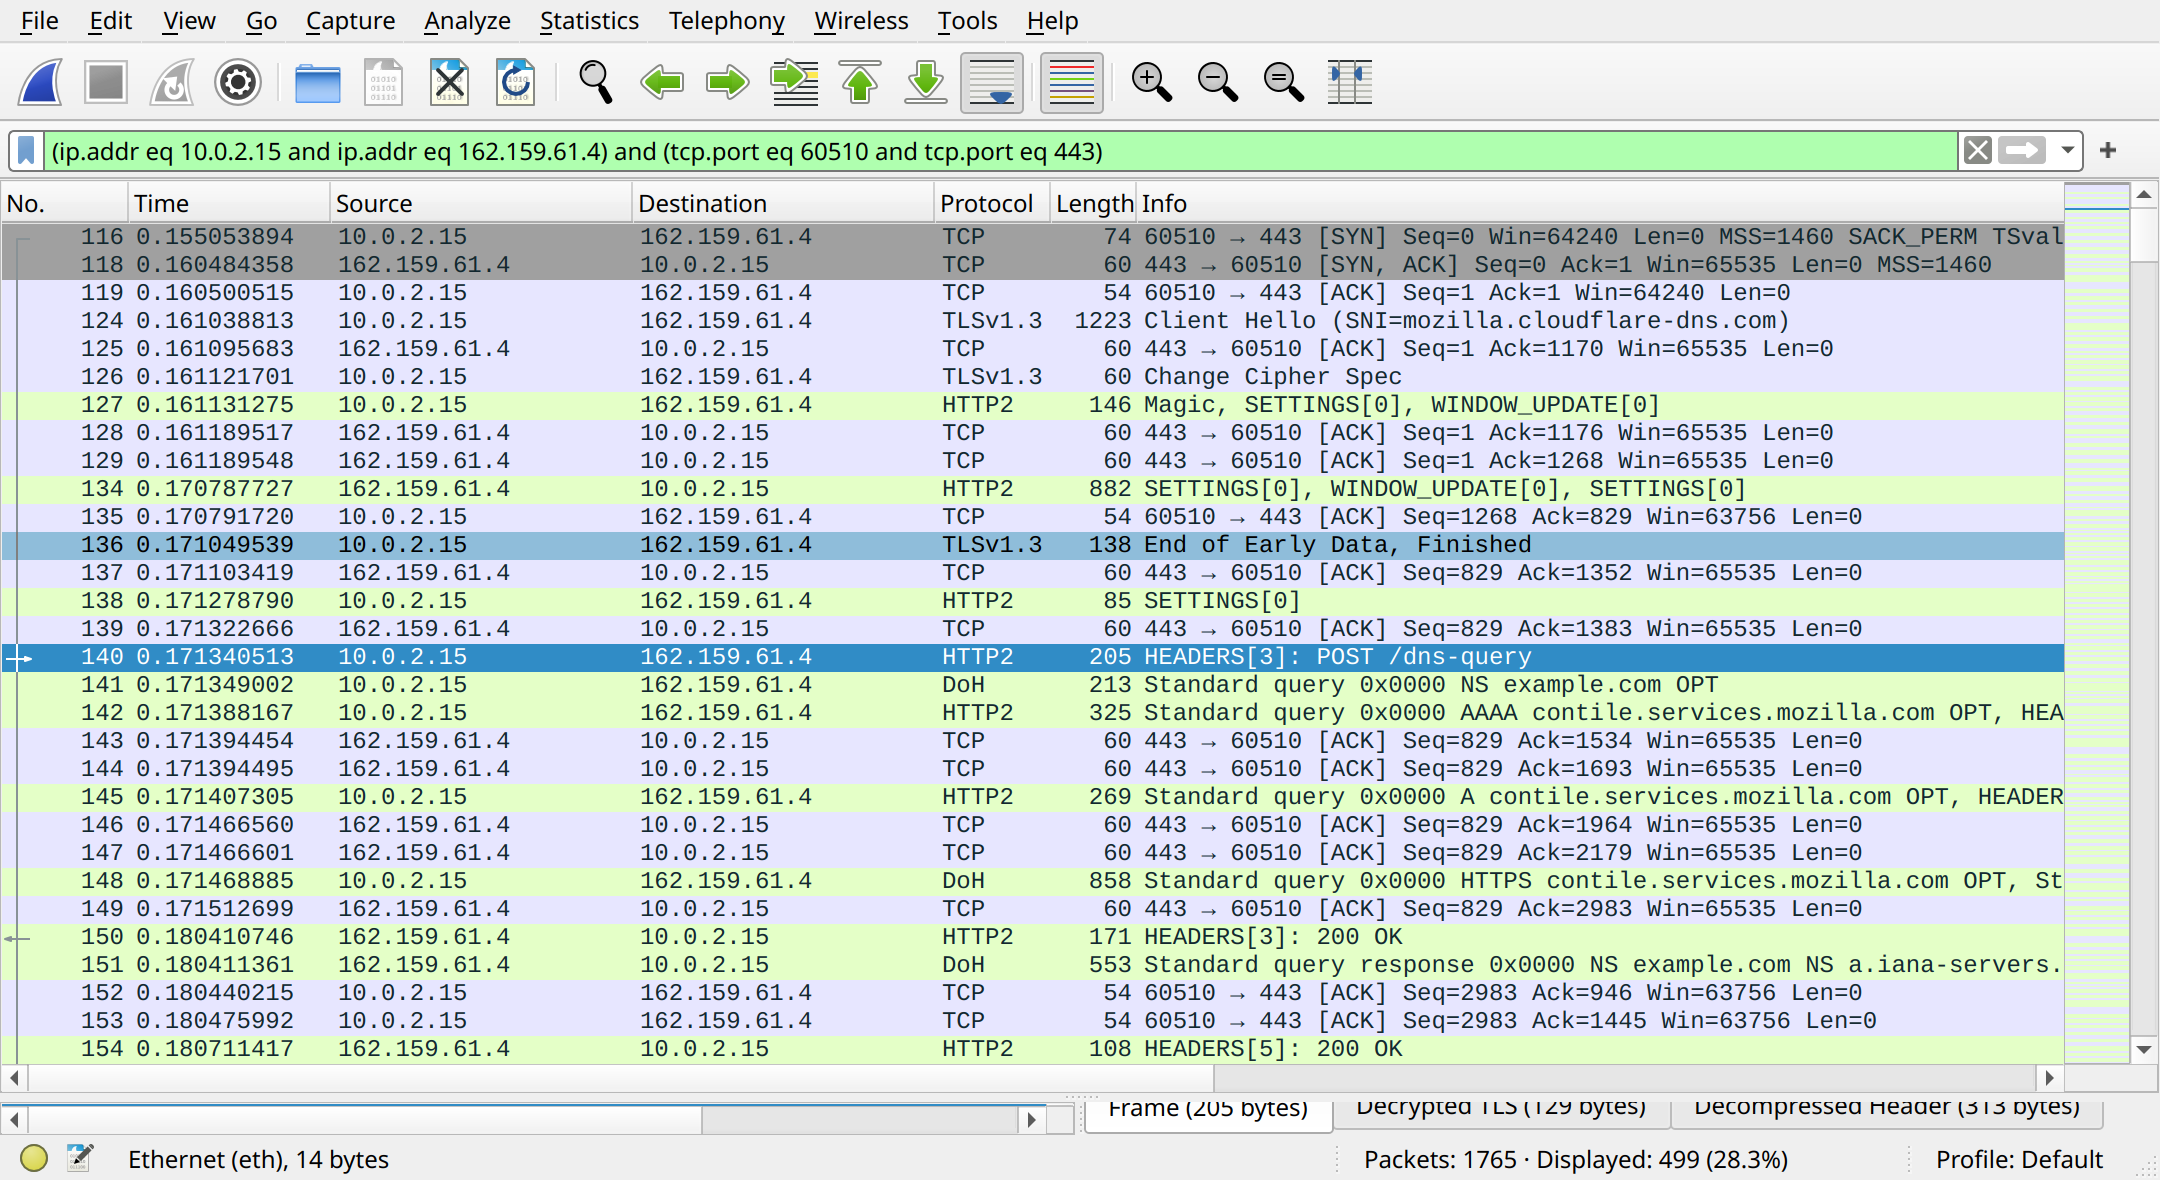
\includegraphics[width=\textwidth]{../intro/wireshark-filtered.png}
};
\path (0, 0) rectangle (14.5, -7); % for bounding box
\draw[overlay,help lines] (0, 0) grid (14, -8);
\draw[overlay,help lines,dotted] (0, 0) grid[step=0.2] (14, -8);
\begin{visibleenv}<1>
    \path[draw, red, very thick] (0.3, -0.9) rectangle (13.15, -1.15);
    \node[anchor=north,overlay box,text=red] (filter expr label) at (6.5, -1.15) {
        filter expression 
    };
    \node[anchor=north,overlay box,font=\fontsize{10}{11}\selectfont,align=left] at (filter expr label.south) {
        based on address ($\sim$ machine) and port number ($\sim$ program/socket) fields  \\
        usually means all part of one socket connection
    };
    \path[draw, red, very thick] (10.3, -7.6) rectangle (12.1, -7.9);
    \node[anchor=south,overlay box,text=red] at (11.4, -7.6) {
        499 packets in ``conversation''
    };
\end{visibleenv}
\begin{visibleenv}<2>
    \path[draw,red, very thick] (0, -1.9) rectangle (.85, -2.24);
    \path[draw,red, very thick] (0, -3) rectangle (.85, -3.37);
    \node[overlay box,anchor=west,text=red] at (.85, -2.5) {
        some packets not shown from filter
    };
\end{visibleenv}
\begin{visibleenv}<3>
    \path[draw,red,very thick] (6.25, -1.47) rectangle (7.1, -7.2);
    \node[align=left,overlay box,anchor=south east,text=red] at (6.25, -3) {
        highest layer used \\
        in each packet
    };
    \node[align=left,overlay box,anchor=north east,text=black,font=\fontsize{10}{11}] at (6.25, -3) {
        connection only `for' \\
        DNS over HTTPS (DoH) \\
        but many packets \\
        only needed for \\
        bookkeeping for \\
        the `lower' layers
    };
\end{visibleenv}
\begin{visibleenv}<4>
    \path[draw,red,very thick] (2.2, -1.47) rectangle (6.25, -7.2);
    \node[align=left,overlay box,anchor=west] at (6.25, -4) {
        bookkeeping packets sent \\
        in both directions
    };
\end{visibleenv}
\end{tikzpicture}
\end{frame}
